\let\negmedspace\undefined
\let\negthickspace\undefined
\documentclass[journal]{IEEEtran}
\usepackage[a5paper, margin=10mm, onecolumn]{geometry}
\usepackage{lmodern} % Ensure lmodern is loaded for pdflatex
\usepackage{tfrupee} % Include tfrupee package

\setlength{\headheight}{1cm} % Set the height of the header box
\setlength{\headsep}{0mm}     % Set the distance between the header box and the top of the text

\usepackage{gvv-book}
\usepackage{gvv}
\usepackage{cite}
\usepackage{amsmath,amssymb,amsfonts,amsthm}
\usepackage{algorithmic}
\usepackage{graphicx}
\usepackage{textcomp}
\usepackage{xcolor}
\usepackage{txfonts}
\usepackage{listings}
\usepackage{enumitem}
\usepackage{mathtools}
\usepackage{gensymb}
\usepackage{comment}
\usepackage[breaklinks=true]{hyperref}
\usepackage{tkz-euclide} 
\usepackage{listings}
\def\inputGnumericTable{}                                 
\usepackage[latin1]{inputenc}                                
\usepackage{color}                                            
\usepackage{array}                                            
\usepackage{longtable}                                       
\usepackage{calc}                                             
\usepackage{multirow}                                         
\usepackage{hhline}                                           
\usepackage{ifthen}                                           
\usepackage{lscape}

\begin{document}

\bibliographystyle{IEEEtran}
\vspace{3cm}

\title{6.5.16}
\author{EE24BTECH11002 - Agamjot Singh}
% \maketitle
% \newpage
% \bigskip
{\let\newpage\relax\maketitle}

\renewcommand{\thefigure}{\theenumi}
\renewcommand{\thetable}{\theenumi}
\setlength{\intextsep}{10pt} % Space between text and floats
prim
\textbf{Question:}
\newline
Find two positive numbers whose sum is $16$ and the sum of whose cubes is minimum.
\textbf{Solution:}

\textbf{Theoritical solution:}
\newline
Let the two numbers be $x$ and $y$, $x$, $y \geq 0$.
It is given that, 
\begin{align}
    x + y = 16
\end{align}
and we have to minimize
\begin{align}
    f\brak{x, y} = x^3 + y^3, \text{, } x, y > 0
\end{align}
Writing $y$ in terms of $x$, we get,
\begin{align}
    f\brak{x} &= x^3 + \brak{16 - x}^3 = 3x^2 - 48x + 256\label{f} \text{, } 0 < x < 16\\
    f^{\prime}\brak{x} &= 3x^2 - 3\brak{16 - x}^2\\
    f^{\prime\prime}\brak{x} &= 6x + 6\brak{16 - x}
\end{align}
For a minimum to occur, $f^{\prime}\brak{x} = 0$ and $f^{\prime\prime}\brak{x} > 0$,
\begin{align}
    f^{\prime}\brak{x} &= 0\\
    \implies 3x^2 - 3\brak{16 - x}^2 &= 0\\
    \implies x &= 8
\end{align}
To verify if it is a minimum, 
\begin{align}
    f^{\prime\prime}\brak{8} &= 96 > 0\\
    \implies x &= 8 \text{, } y = 16 - x = 8 \text{ is where the minimum occurs}\\
    \implies f_{\text{min}} &= 8^3 + 8^3 = 1024
\end{align}
\newline
\textbf{Computational Solution:} Gradient Descent algorithm
\newline
By the gradient descent algorithm, the difference equation is given by,
\begin{align}
    x_{n + 1} = x_n - \mu f^{\prime}\brak{x}\\
    \implies x_{n + 1} = x_n - \mu \brak{6x_n - 48}\\
    \implies x_{n + 1} = \brak{1 - 6\mu}x_n + 48\mu \label{diff_eq}
\end{align}
where $f$ is the objective function given by equation \brak{\ref{f}} and $\mu > 0$ is the step size.
Taking one sided $Z$-transform on both sides of \brak{\ref{diff_eq}},
\begin{align}
    zX\brak{z} - zx_0 &= \brak{1 - 6\mu}X\brak{z} + 48\mu\\
    \brak{z + 6\mu - 1}X\brak{z} &= 48\mu + zx_0\\
    X\brak{z} &= \frac{48\mu + zx_0}{z + 6\mu - 1}\\
    X\brak{z} &= \frac{48\mu z^{-1}}{1 + \brak{6\mu - 1}z^{-1}} + \frac{x_0}{1 + \brak{6\mu - 1}z^{-1}}\\
    X\brak{z} &= 48\mu \sum_{n = 0}^{\infty} \brak{1 - 6\mu}^{n} z^{-\brak{n + 1}} + x_0\sum_{n = 0}^{\infty} \brak{1 - 6\mu}^{n} z^{-n}\\
    X\brak{z} &= \brak{48\mu z^{-1} + x_0} \sum_{n = 0}^{\infty} \brak{1 - 6\mu}^{n} z^{-n} \label{ztrans_eq}
\end{align}
By \brak{\ref{ztrans_eq}}, ROC is given by,
\begin{align}
    \abs{\frac{1 - 6\mu}{z}} &< 1\\
    \implies \abs{z} &> \abs{1 - 6\mu}\\
    \implies \abs{1 - 6\mu} &> 0\\
    \implies \mu &\in \mathbb{R} \setminus \cbrak{\frac{1}{6}}
\end{align}

If the sequence $x_n$ has to converge,
\begin{align}
    \lim_{n\to\infty} \abs{x_{n + 1} - x_n} &= 0\\
    \implies \lim_{n\to\infty} \abs{-6\mu x_n + 48\mu} &= 0\\
    \implies \mu \lim_{n\to\infty} \abs{-6x_n + 48} &= 0 \text{, } \mu > 0\\
    \implies \lim_{n\to\infty} x_n = 8
\end{align}

We take the initial guess $= 7$, step size $= 0.01$, tolerance $= 0.0001$.
\newline
Scipy Solution:
\newline
\begin{align}
    f_{\text{min}} = 1024.0000000000005\text{, } x_{\text{min}} = 7.999999930756325
\end{align}
\newline
Using the gradient descent algorithm, we get,
\begin{align}
    f_{\text{min}} = 1024.000000004813\text{, } x_{\text{min}} = 7.999989986419678
\end{align}

\begin{figure}[h!]
   \centering
   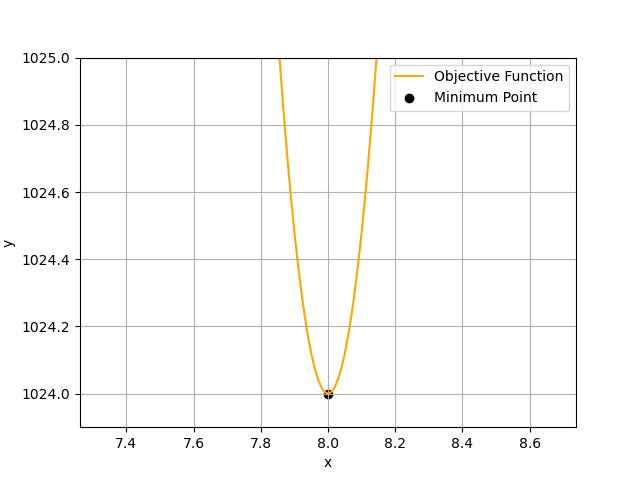
\includegraphics[width=0.7\columnwidth]{figs/graph.png}
   \caption{Objective Function with the minimum point}
   \label{label}
\end{figure}

\end{document}
